%!TEX root = ../../thesis.tex

\chapter{Reassortment in Influenza Evolution}
\label{ch:influenza}

\section{Introduction}
\label{flu:introduction}

In this chapter, we study influenza virus, a common human pathogen with a substantial burden on human health.
Seasonal influenza epidemics have an annual mortality of between 250,000 and 500,000 \cite{WHO:2014b}.
Influenza pandemics, which have historically occurred roughly once every thirty years, can infect between 20-40\% of the global population.
For example, the Spanish influenza pandemic of 1918-1919 is estimated to have infected approximately 500 million people and lead to the death of between 50-100 million people \cite{Taubenberger:2006kl}.
This amounts to an infection of approximately 33\% of the population and a case fatality ratio of 5-6\% of global population.

The natural host reservoir of influenza is waterfowl.
Within this reservoir, several distinct subtypes circulate.
Subtypes are labeled by the antigenic type of two surface proteins, hemagglutinin (HA) and neuraminidase (NA).\footnote{An antigen is a molecule that elicits a host immune response. The adaptive immune system learns to recognize an antigenic type. Antigenic variation occurs when sufficient genomic alteration has occurred for a protein to evade the immune response.}
There are presently eighteen types of HA (H1 to H18) and eleven types of NA (N1 to N11).
Zoonotic adaptations have led to multiple introductions to human populations, which have resulted in both isolated outbreaks and sustained transmission \cite{Nelson:2007bc}.\footnote{Understanding the genetic basis for host adaptation is an important and controversial research area. Our work in this area in collaboration with Yoshihiro Kawaoka is forthcoming \cite{Walters:2016a}.}

The evolution of influenza is punctuated by frequent reassortment.
Reassortment occurs when two virus particles coinfect the same host cell, and is a consequence of influenza having a segmented genome.
The result is viral progeny that carries genomic information from two independent parental strains.
This mode of evolution is known as \emph{antigenic shift}, because it can rapidly lead to antigenically distinct viral strains.\footnote{As opposed to \emph{antigenic drift}, due to random mutation and genetic drift.}
Antigenic shifts have historically been the cause of major pandemics, which can occur when novel surface proteins reassort with internal segments already adapted to the human host.
Reassortments of this type led to Asian flu pandemic of 1957 and the Hong Kong flu pandemic of 1968 \cite{Lindstrom:2004il}.
The 2009 H1N1 pandemic strain emerged from a triple reassortment between avian, swine, and human circulating strains \cite{Hernandez:2011ud,Smith:2009io}.
The pandemic had a global infection rate of between 11\%-21\% but a lower mortality rate than initially expected.\footnote{The 2009 H1N1 pandemic is an excellent example of the delicate balance between virulence and transmissibility.}
The 2013 H7N9 outbreak was caused by a triple reassortment of three distinct avian strains \cite{Chen:2013kp}.
Traditionally, reassortments have been identified by hand by comparing phylogenetic trees constructed from different genomic segments \cite{Nelson:2006bx}.

Recent years have seen increased concerns about the pandemic potential for zoonotic adaptation of highly pathogenic strains of influenza.
Of particular concern is H5N1, which has an estimated case fatality rate of 50\% (449 deaths from 846 confirmed human cases) \cite{WHO:2016a}, but has so far not exhibited sustained person-to-person transmission \cite{WHO:2014b}.
These concerns underscore the need to efficiently characterize and represent reticulate evolution in influenza.
Since the 2009 H1N1 pandemic, substantial effort has been put into collected fully sequenced influenza genomes.
The NCBI Influenza Virus Resource now contains over 400,000 unique viral isolates \cite{Bao:2008cq}.
The large quantity of genomic data that has been collected provides an ideal environment for studying reticulate evolution with high resolution.

\section{Influenza Virology}
\label{flu:virology}

Influenza is an enveloped single-stranded negative-sense RNA virus of family Orthomyxoviridae.
The virus has a segmented genome with eight segments coding for eleven proteins.
The genome length is approximately 13.5~kb.
The viral structure is shown in Figure~\ref{fig:flu:genome}.
The segments are typically ordered from longest to shortest and are detailed in Table~\ref{table:influenza_genome_segments}.
Of these segments, hemagglutinin (HA) and neuraminidase (NA) are the two most important.
HA and NA form the two surface protein markers and 
On the surface of the viral particle are HA and NA.
HA regulates host cell binding and entry into host epithelial cells.
HA is the strongest determinant of host specificity: different hosts express different sialic acid types.
Avian influenza binds to type 2-3 sialic acid receptors, while human influenza binds to type 2-6 sialic acid receptors.
NA is the surface protein that cleaves the newly replicated virus particles from the cell surface.
Together, HA and NA determine the strain subtype and are a primary marker of host transmission and specificity.
Both are antigens.
PA, PB1, and PB2 form a polymerase complex and are involved in viral replication.
Mutations in these proteins can be among the most important in determining host adaptation and virulence.
The remaining proteins, including NP, M1, M2, and NS1 are largely structural proteins involved in capsid formation and viral packaging.

\begin{table}
\centering
\caption{Influenza Genome Segments}
\small
\rowcolors{2}{gray!25}{white}
\setlength{\aboverulesep}{0pt}
\setlength{\belowrulesep}{0pt}
\setlength{\extrarowheight}{.75ex}
\begin{tabularx}{\textwidth}{XXXXX}
\toprule\rowcolor{gray!50}
Segment & Length (aa) & Name & Abbreviation & Proteins \\
\midrule
1 & xx & Polymerase basic 2 & PB2 & PB2 \\
2 & xx & Polymerase basic 1 & PB1 & PB1,PB1-F2 \\
3 & xx & Polymerase acidic & PA & PA \\
4 & xx & Hemagglutinin & HA & HA \\
5 & xx & Nucleoprotein & NP & NP \\
6 & xx & Neuraminidase & NA & NA \\
7 & xx & Matrix        & M  & M1,M2 \\
8 & xx & Nonstructural & NS & NS1 \\
\bottomrule
\end{tabularx}
\label{table:influenza_genome_segments}
\end{table}

\begin{figure}
\begin{center}
\centerline{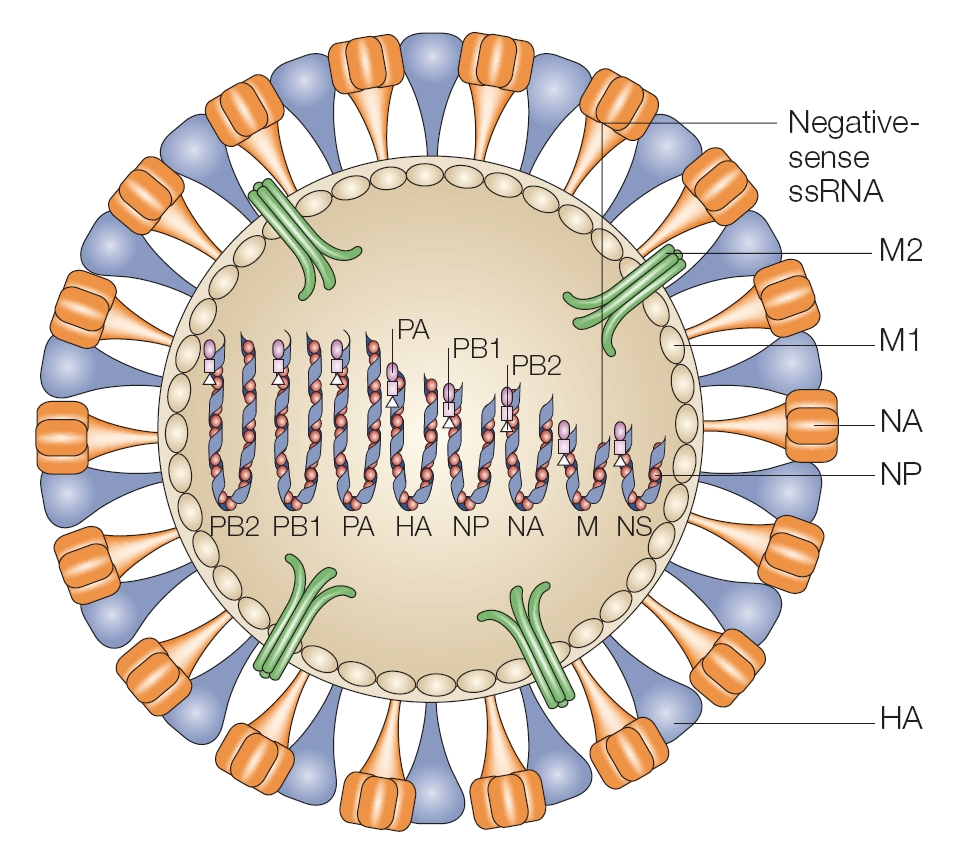
\includegraphics[width=.5\columnwidth]{./fig/influenza/flu_genome.jpg}}
\caption[Structure of an influenza virus particle]{Structure of an influenza virus particle. Surface antigens HA and NA coat this surface and are involved in cell entry and exit. The surface capsid is formed from matrix proteins M1 and M2. PB1, PB2, and PA form a polymerase complex assisting in viral replication in the infected cell.}
\label{fig:flu:genome}
\end{center}
\end{figure}

\section{Influenza Reassortment}
\label{flu:reassortment}

We characterized reassortment in avian influenza using persistent homology.
We first compiled an aligned dataset of 3,105 complete avian influenza genomes from the NIH Influenza Sequence Database.
These sequences span in time from 1956 to 2012. 
We collected samples from all influenza subtypes.
The distribution of collected HA types is shown in Figure~XX.
The majority of our sequences are of the H5 and H6 type, with a smaller proportion of H3, H7, and H9.

We first applied persistent homology to each genomic segment individually, as shown in Figure~\ref{fig:flu:segment_barcodes}.
Here we see broadly only zero-dimensional homology, consistent with no intra-segmental recombination.
The presence of higher homology is likely due to back mutation, which is expected to be more common in viruses with high mutation rates and shorter genomes (i.e. the infinite sites model does not hold).
However, an analysis of the concatenated full genome reveals a complex topology, with a large number of homological invariants in one and two dimensions.

In settings of vertical evolution, we can directly transform a filtration of 0-D simplicial complexes into an equivalent distance-based dendrogram.
Fig. 2A represents the zero-dimensional topology of the hemagglutinin segment of avian influenza viruses. 
The zero-dimensional generators at higher genetic distances indicate the major clusters, coinciding with the antigenic subtypes H1-H16.
From the bar sizes of the barcode plot, we can create a dendrogram that recapitulates classic phylogenetic analyses (Fig. 2B).
Only when segments are concatenated does persistent homology indicate that reassortment precludes phylogenetic analysis (Fig. 2C).
These results show that persistent homology can detect pervasive reassortment in influenza.
Estimating ICR from one-dimensional homology provides a lower-bound on reassortment rate in influenza.
We calculate an ICR of <1 event per year for classic H1N1 swine and H3N2 human influenza viruses, supported by previous phylogenetic estimates.
In contrast, we calculate a high reassortment rate of 22.16 events per year for avian influenza A.
This difference could be explained by the high diversity and frequent co-infection of avian viruses and correlates with the high proportion of potential avian reassortants reported in previous studies.

To illustrate how higher-dimensional topology captures reassortments, we analyzed 1,000 human H3N2 genomes and identified three generators of one-dimensional homology when joining the PB2 and HA segments.
As an example, the [G3] generator with the longest bar (Dataset S1, Table S5) is represented by an oriented one-dimensional irreducible cycle, implying at least one reassortment involving PB2 and HA of the isolates or their ancestors.
The number of sequences in the generator serves as an upper bound on the number of candidate reassortants.
Simple observation of the resulting sequence alignment reveals two divergent allelic patterns between informative sites in PB2 and HA, as reflected in incongruent trees (SI Appendix, Fig. S8 A and B) and reticulate cycles of the phylogenetic network (SI Appendix, Fig. S8C).

One-dimensional $\ICR$ provides a lower-bound estimate of reassortment rate (SI Appendix, Fig. S10B).
We calculate $\ICR < 1$ event per year for classic H1N1 swine and H3N2 human influenza, supported by previous phylogenetic estimates \cite{Lycett:2012fqa,Holmes:2005cia}.
In contrast, we calculate a high rate of 22.16 reassortments per year for avian influenza A (Dataset S1, Table S16).
This difference could be explained by the high diversity and frequent coinfection of avian viruses \cite{Lubeck:1979ws} and correlates with the high proportion of avian reassortants reported in previous studies \cite{Dugan:2008iba}.

\begin{figure}
\centering
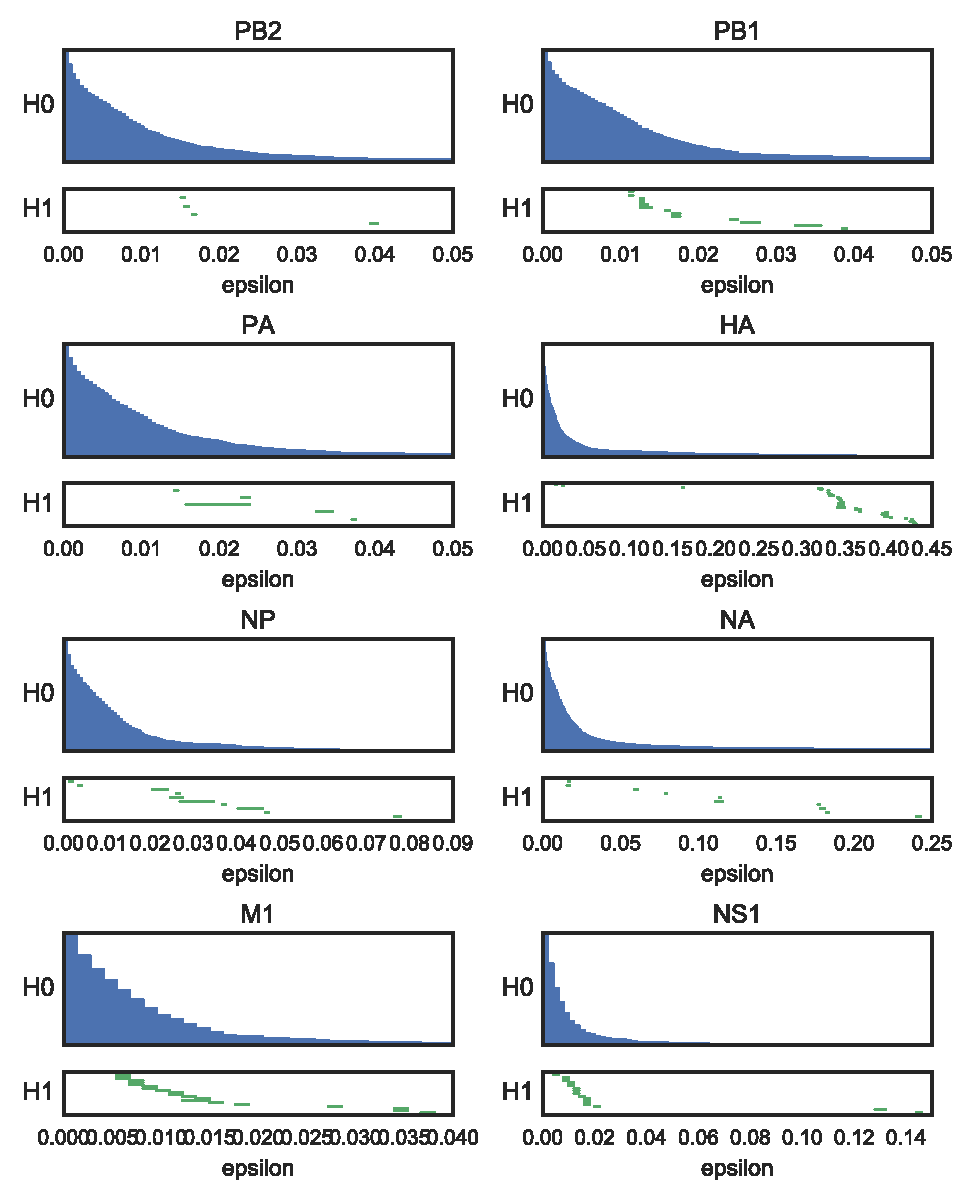
\includegraphics[]{fig/influenza/flu_segment_barcodes.pdf}
\caption[Influenza Segment Barcodes]{Influenza Segment Barcodes. Very little $H_1$ present.}
\label{fig:flu:segment_barcodes}
\end{figure}

\begin{figure}
\centering
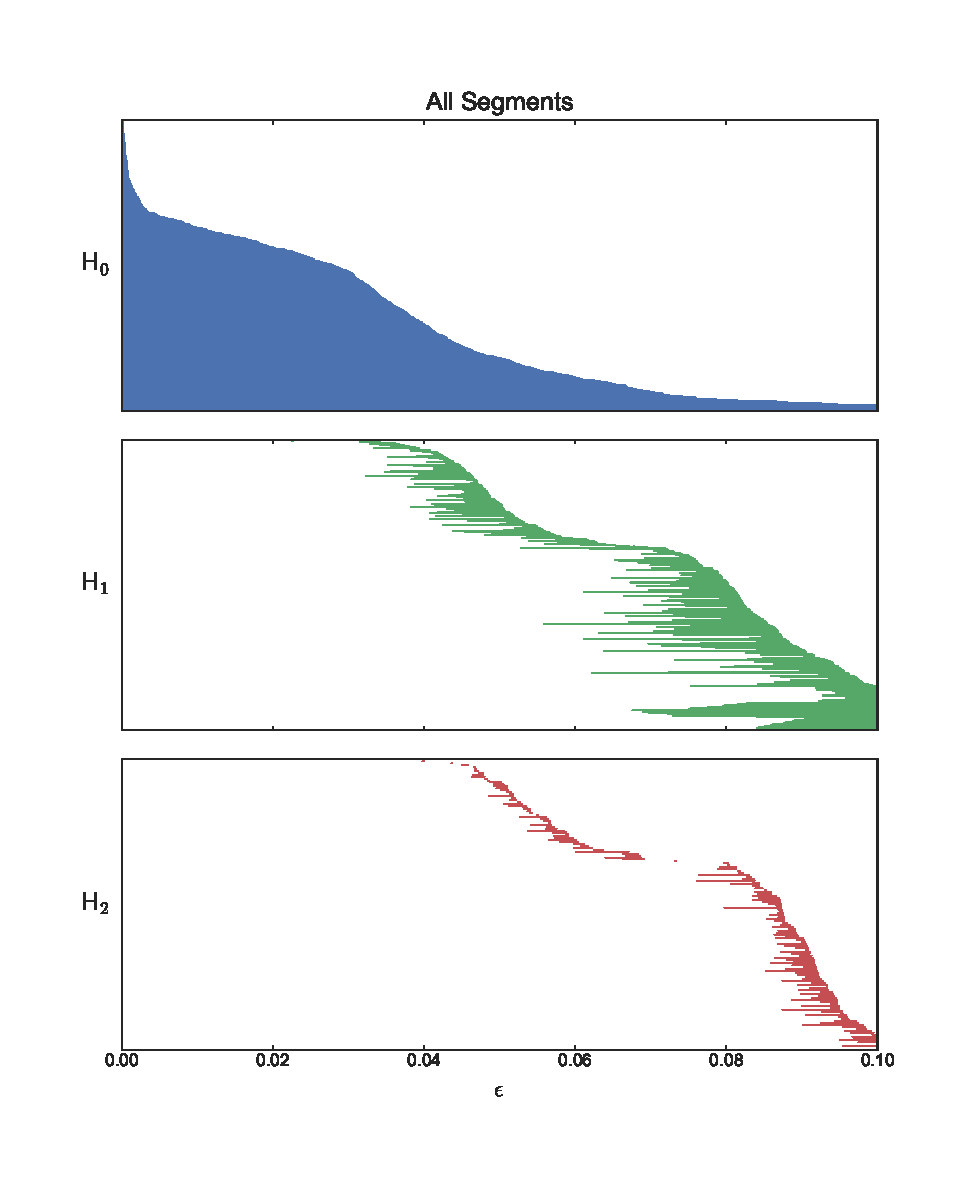
\includegraphics[]{fig/influenza/flu_concat_barcode.pdf}
\caption[Influenza Concatenated Genome Barcode]{Influenza Concatenated Genome Barcode}
\label{fig:flu:concatenated_genome_barcode}
\end{figure}

We used mapper to visualize the relationships in our influenza dataset.
A series of mapper networks is shown in Figure~\ref{fig:flu:networks_by_subtype}.
The networks were generated using a Hamming metric and the first and second MDS component as a 2d lens.
In each subfigure we color the network by the prevalence of each HA subtype in the particular node.
It is interesting to note how this is different than a traditional phylogeny based on HA.

\begin{figure}
\centering
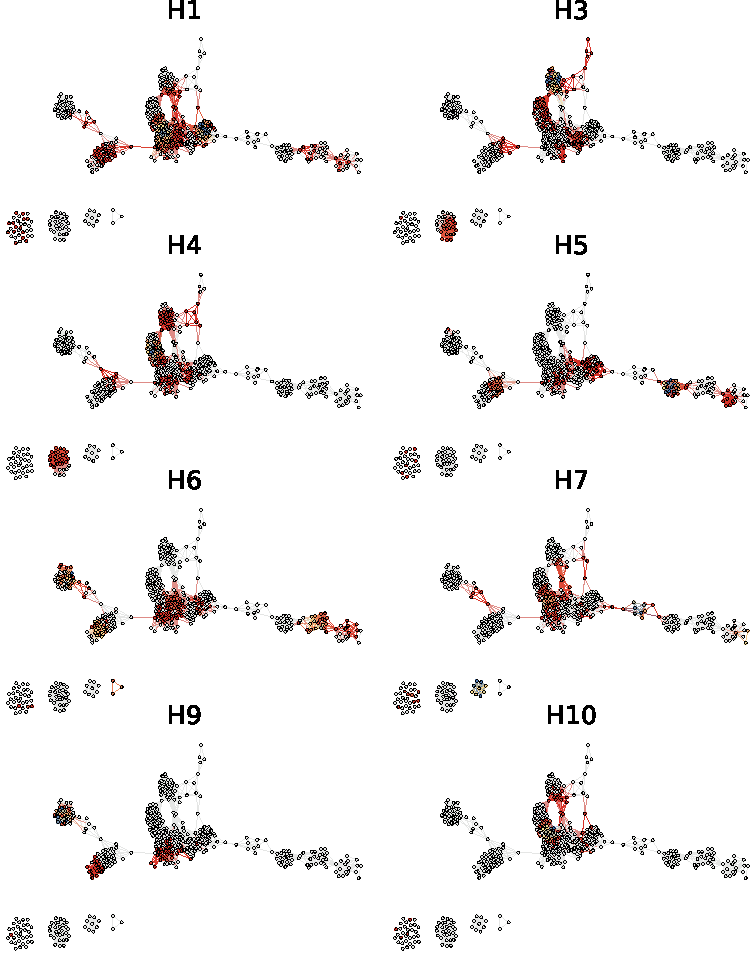
\includegraphics[width=\textwidth]{fig/influenza/flu_networks_by_subtype.pdf}
\caption[Influenza Networks By HA Subtype]{Influenza Networks By HA Subtype. The networks were generated using Ayasdi. }
\label{fig:flu:networks_by_subtype}
\end{figure}

\section{Nonrandom Association of Genome Segments}
\label{flu:nonrandom_reassortment}

% (This section needs more details)
We observed nonrandom association of flu segments.
Statistical inference on the loops corresponding to reassortments identified segments that tend to co-segregate with each other during reassortment.In particular, polymerases co-segregate, while genes coding for envelope and capsid proteins show independent reassortment patterns.
Cosegregation of polymerases suggests that effective protein–protein interaction between the polymerase complex and the NP protein constrain reassortment. 

Although previous phylogenetic studies confirmed a high reassortment rate in avian influenza, none has identified a clear pattern of gene segment association \cite{Dugan:2008iba}.
To determine whether any segments cosegregate more than expected by chance, we applied persistent homology to avian influenza.
We first considered all pairs of concatenated segments and estimated the number of reassortments by $b1$.
We then ascertained the significance of observing a number of reassortments between each pair of segments given the total estimate of reassortments in the concatenated genome (SI Appendix, Supplementary Text).
Analysis of avian influenza reveals a statistically significant configuration of four cosegregating segments: polymerase basic 2 (PB2), polymerase basic 1 (PB1), polymerase acidic (PA), and nucleoprotein (NP) (Fig. 3D).
Interestingly, this pattern mimics previous in vitro results that suggest that effective protein-–protein interaction between the polymerase complex and the NP protein constrain reassortment \cite{Lubeck:1979ws}.

\begin{figure}
\begin{center}
\centerline{
\includegraphics[width=\columnwidth]{./fig/influenza/flu_reassortment_correlations.pdf}}
\caption[Influenza Nonrandom Reassortment]{Influenza Nonrandom Reassortment}
\label{fig:flu:nonrandom_reassortment}
\end{center}
\end{figure}

\section{Multiscale Flu Reassortment}
\label{flu:multiscale_reassortment}

We computed persistent homology on an aligned dataset of 3,105 avian influenza sequences across the seven major HA subtypes.
The persistence diagram is shown in Figure \ref{fig:flu:scatterplot}, along with density estimates for the birth and death distributions.
Both birth and death times appear strongly bimodal, unlike in the coalescent simulations, which were strictly unimodal.
This suggests two distinct scales of topological structure.
Using the representative cycles output by Dionysus on a subset of this data, we classified features as intrasubtype (involving one HA subtype) and intersubtype (involving multiple HA subtypes).
The $H_1$ barcode diagram for this data is shown in the Figure \ref{fig:flu:scatterplot} inset.
Intrasubtype features, in blue, occur at an earlier filtration scale than intersubtype features, in green.
The multiscale topological approach of persistent homology can distinguish biological events occuring at different genetic scales.

We isolated the two peaks and estimated two recombination rates: an intrasubtype $\rho_{1}=9.68$, and an intersubtype $\rho_{2}=21.43$.
We conclude that intersubtype recombination occurs at a rate over twice that of intrasubtype recombination, however a genetic barrier exists that maintains distinct subtype populations.
The nature of this barrier warrants further study.
This illustrates a real world example in which multiscale topological structure can be captured by persistent homology and given biological interpretation.

% figure
\begin{figure}
\begin{center}
\centerline{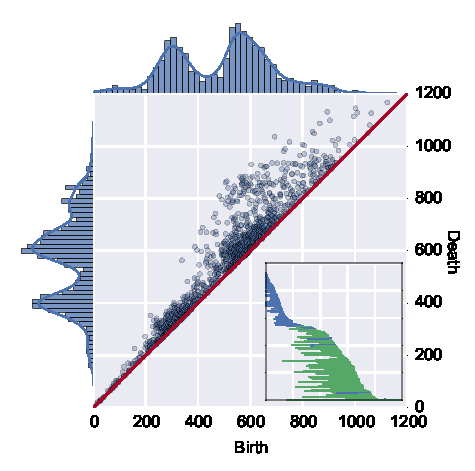
\includegraphics[width=\columnwidth]{./fig/influenza/flu_scatterplot.pdf}}
\caption[$H_1$ persistence diagram computed from an avian influenza dataset.]{The $H_1$ persistence diagram computed from an avian influenza dataset. On the top and left are plotted the marginal distributions of birth and death times, along with a density estimate for each distribution. The bimodality indicates two scales of topological structure. Inset: The barcode diagram for a subset of this data. Blue bars have representative cycles involving only one subtype, green bars have cycles involving multiple subtypes.}
\label{fig:flu:scatterplot}
\end{center}
\end{figure}

\section{Prediction of Host Specific Residues}
\label{flu:flumarker}

In this section, we describe work in prediction of host specific residues using machine learning approaches.
Host specific residues are important for viral surveillance in order to predict possible outbreaks.
We describe here two methods and include preliminary validation from our collaborator in Wisconsin.

\section{Conclusions}
\label{flu:conclusions}

The segmented nature of the influenza genome makes it an ideal 
Coinfection of a single cell by 
Coinfection of a single cell with multiple strains of influenza can lead to genomic reassortment.
Reassortments can lead to novel pandemics.
Therefore it is important that methods to characterize reassortment be developed.
In this chapter we have applied methods from TDA to characterize reassortment in influenza.
Using our approach, we have confirmed that intrasegmental recombination does not occur.
We have estimated reassortment rates.
We have estimated recombination rates.
Further, from the persistence diagram we identified a bimodal presence of $H_1$ invariants.
This suggests a genetic barrier maintaining subtype diversity.




